\section{Finite topology as primitive recursive mathematics}\label{sec:finite}

This section proves twenty-four uniform finite theorems.  They address the
entries on topology, exterior, homeomorphisms, compact-open topology,
Urysohn separation and metrization, together with finite forms of the
discrete-family terminology.  The restriction is on the \emph{represented
objects}, not on the sizes of the finite instances: the proofs are uniform
in every natural-number carrier size.  All subsets here have Boolean
codes.  Consequently bounded searches, complement formation, and
case distinctions on membership are legitimate in \ipra.  Nothing in
this section turns an arbitrary infinite predicate into a decidable set.

\subsection{Codes and the specialization relation}

Put $[n]=\{0,\ldots,n-1\}$.  A subset $A\subseteq[n]$ is represented by
the integer $a<2^n$ whose $x$th binary digit is its membership bit.  A
relation is represented by $r<2^{n^2}$; write $x\preceq y$ when bit
$nx+y$ is one.  Its validity conditions are the bounded statements
\[
 (\forall x<n)\ x\preceq x,\qquad
 (\forall x,y,z<n)\bigl(x\preceq y\land y\preceq z
                         \Rightarrow x\preceq z\bigr).
\]
They define a \emph{preorder}; antisymmetry is not required.  A topology
table is a mask of length $2^n$: its bit at $a$ says whether the subset
with code $a$ is open.  A map $[n]\to[m]$ is a length-$n$ table of
entries below $m$.  Empty carriers cause no exception: there is one
empty table, and there is no map from a nonempty carrier to the empty
one.

For a preorder define
\[
 \mathord\uparrow x=\{y:x\preceq y\},\qquad
 \mathord\downarrow x=\{y:y\preceq x\}.
\]
A set $U$ is \emph{upward closed} if $x\in U$ and $x\preceq y$ imply
$y\in U$; downward closed has the reversed implication.  The chosen
orientation is important: open sets will be upward closed, and the
closure of $\{x\}$ will be $\mathord\downarrow x$.

\begin{theorem}[F01: topology from a preorder]\label{thm:finite-upsets}
The upward-closed subsets of a finite preorder form a topology.
The least open neighborhood of $x$ is $\mathord\uparrow x$, and these
$n$ sets form a basis.  Every open set $U$ satisfies
$U=\bigcup_{x\in U}\mathord\uparrow x$.
\end{theorem}
\begin{proof}
The empty and full sets are upward closed.  If $x$ belongs to both of
two upward-closed sets, every $y$ above $x$ belongs to both; hence their
intersection is upward closed.  If $x$ belongs to a member of a coded
family, that same member contains every $y$ above $x$; its union is
therefore upward closed.  Transitivity makes
$\mathord\uparrow x$ upward closed, reflexivity puts $x$ in it, and
the definition of upward closure places it in every open neighborhood
of $x$.  These observations prove the displayed union identity.
For the finite topology table, closure under binary unions already
gives closure under every finite list by a bounded fold.  No code for
an unbounded union is required.
\end{proof}

\begin{theorem}[F02: recovery of every finite topology]\label{thm:finite-recover}
Suppose a table $\mathcal T$ contains the empty and full subsets and
is closed under binary intersection and union.  Define
\[
 x\preceq_{\mathcal T}y
 \quad\Longleftrightarrow\quad
 (\forall U\in\mathcal T)\ (x\in U\Rightarrow y\in U).
\]
This is a preorder, and its upward-closed subsets are exactly
$\mathcal T$.  Starting with a preorder and performing this recovery
returns the original relation.
\end{theorem}
\begin{proof}
Reflexivity and transitivity follow by substituting the same open set
into the defining implications.  Let $N_x$ be the intersection of
the at most $2^n$ listed opens containing $x$.  This nonempty list
includes $[n]$, so a bounded fold computes $N_x\in\mathcal T$.
Its elements are exactly the $y$ with $x\preceq_{\mathcal T}y$.
Every listed open is upward closed by definition.  Conversely, an
upward-closed $U$ is the union of $N_x$, $x\in U$, so belongs to
$\mathcal T$ by binary-union closure.  Finally, for an initial
preorder, $x\preceq y$ implies membership of $y$ in every upward
set containing $x$.  If the recovered relation holds, apply it to
the upward set $\mathord\uparrow x$ to recover $x\preceq y$.
All quantifiers in this construction run over bounded mask ranges.
\end{proof}

\subsection{Interior, closure, exterior, and boundary}

\begin{theorem}[F03: explicit interior and closure]\label{thm:finite-intcl}
For every coded subset $A$,
\[
 \operatorname{Int}A=\{x:(\forall y<n)(x\preceq y\Rightarrow y\in A)\},
 \qquad
 \operatorname{Cl}A=\{x:(\exists y<n)(x\preceq y\land y\in A)\}.
\]
The first is the greatest open subset of $A$, and the second is the
least closed superset of $A$.  Here closed subsets are exactly the
downward-closed subsets.
\end{theorem}
\begin{proof}
A complement is upward closed exactly when the original set is
downward closed, by decidable membership.  Reflexivity shows
$\operatorname{Int}A\subseteq A\subseteq\operatorname{Cl}A$.
If $x$ satisfies the universal condition and $x\preceq z$, then
every $y$ above $z$ is above $x$, so $z$ also satisfies it.  Thus the
interior formula defines an open set.  If $U$ is open and
$U\subseteq A$, every point above $x\in U$ remains in $U$ and hence
in $A$; therefore $U\subseteq\operatorname{Int}A$.
If $z\preceq x$ and $x\preceq y\in A$, transitivity gives
$z\preceq y\in A$, proving that the closure formula is downward
closed.  Any downward-closed $D\supseteq A$ contains such $x$, so it
contains $\operatorname{Cl}A$.  Both formulas are evaluated by loops
of length at most $n^2$.
\end{proof}

\begin{theorem}[F04: closure and interior laws]\label{thm:finite-laws}
Interior and closure are monotone and idempotent.  Moreover,
\[
\begin{split}
 \operatorname{Int}(A\cap B)&=\operatorname{Int}A\cap\operatorname{Int}B,\\
 \operatorname{Cl}(A\cup B)&=\operatorname{Cl}A\cup\operatorname{Cl}B,\\
 \operatorname{Int}(A^c)&=(\operatorname{Cl}A)^c,\qquad
 \operatorname{Cl}(A^c)=(\operatorname{Int}A)^c.
\end{split}
\]
Also $\operatorname{Cl}\varnothing=\varnothing$ and
$\operatorname{Int}[n]=[n]$.
\end{theorem}
\begin{proof}
Monotonicity follows by retaining a universal membership proof or an
existential witness when $A$ is enlarged.  Since the interior is
already open, its greatest-open characterization gives idempotence;
the least-closed characterization gives the dual assertion.  A point
has every successor in $A\cap B$ exactly when every successor is
in each factor.  A successor in $A\cup B$ witnesses one of the two
closure alternatives, and either alternative witnesses the union.
The first complement identity says that no successor lies in $A$;
this is precisely the failure of the existential condition for
closure.  For the second identity, if the bounded universal test
fails, a scan of the $n$ entries returns a successor outside $A$.
This last step uses decidability and finiteness, not a De Morgan
principle for arbitrary predicates.  Empty and full sets follow
directly from the formulas.
\end{proof}

\begin{theorem}[F05: exterior and boundary decomposition]\label{thm:finite-boundary}
Define $\operatorname{Ext}A=\operatorname{Int}(A^c)$ and
$\partial A=\operatorname{Cl}A\cap\operatorname{Cl}(A^c)$.
Then
\[
 [n]=\operatorname{Int}A\ \dot\cup\ \partial A\ \dot\cup\
             \operatorname{Ext}A,
 \qquad
 \partial A=\operatorname{Cl}A\setminus\operatorname{Int}A.
\]
The boundary is closed and $\partial A=\partial(A^c)$.
A subset is both open and closed exactly when its boundary is empty.
\end{theorem}
\begin{proof}
By F04, the exterior is the complement of the closure and
$\operatorname{Cl}(A^c)$ is the complement of the interior.
Since interior is contained in closure, the three indicated Boolean
pieces are disjoint and cover the carrier.  The boundary is an
intersection of closed sets and its definition is symmetric in $A$
and $A^c$.  If $A$ is clopen, its interior and closure are both $A$.
Conversely, empty boundary gives
$\operatorname{Cl}A\subseteq\operatorname{Int}A$; sandwiching $A$
between these sets makes all three equal.
\end{proof}

\subsection{Maps and universal constructions}

\begin{theorem}[F06: continuity is monotonicity]\label{thm:finite-cont}
A map $f:X\to Y$ between finite preorder spaces is continuous
exactly when $x\preceq_X x'$ implies $f(x)\preceq_Y f(x')$.
Identity maps and composites of continuous maps are continuous.
\end{theorem}
\begin{proof}
For a monotone map the inverse image of an upward set is upward:
if $f(x)\in U$ and $x\preceq x'$, then
$f(x)\preceq f(x')$ puts $f(x')$ in $U$.
Conversely, take the open neighborhood
$\mathord\uparrow f(x)$ of $f(x)$.  Its inverse image is open
and contains $x$, so contains every $x'$ above $x$.  This says
$f(x)\preceq f(x')$.  The identity preserves the relation, and
two successive relation-preserving implications prove the composite
claim.  A continuity certificate can therefore be checked using
$|X|^2$ comparisons instead of enumerating all subsets of $Y$.
\end{proof}

\begin{theorem}[F07: the closure criterion]\label{thm:finite-closuremap}
A finite map $f:X\to Y$ is continuous if and only if
\[
 f(\operatorname{Cl}_X A)\subseteq\operatorname{Cl}_Y f(A)
 \quad\hbox{for every coded }A\subseteq X.
\]
\end{theorem}
\begin{proof}
For the forward implication, a witness $x\preceq a\in A$
is carried to $f(x)\preceq f(a)\in f(A)$.
For the converse, if $x\preceq y$, apply the displayed inclusion
to $A=\{y\}$.  The closure of $\{f(y)\}$ consists precisely of
the elements below $f(y)$, so $f(x)\preceq f(y)$; now use F06.
\end{proof}

\begin{theorem}[F08: homeomorphisms and classification]\label{thm:finite-homeo}
A bijection of finite spaces is a homeomorphism exactly when
\[
 x\preceq_X y\quad\Longleftrightarrow\quad f(x)\preceq_Y f(y).
\]
Homeomorphism is an equivalence relation and is decidable for finite
topology tables by a primitive recursive search.
\end{theorem}
\begin{proof}
The two implications are monotonicity of $f$ and of its inverse,
using the inverse table computed by bounded search.  F06 proves the
first assertion.  Identity, inverse, and composition prove
reflexivity, symmetry, and transitivity.  If the carrier sizes differ,
no bijection exists; if they agree, enumerate all $n^n$ tables,
discard those with repeated values, and check the two relation
implications.  This explicit bound suffices; a more efficient
permutation enumeration changes no logical issue.
\end{proof}

\begin{theorem}[F09: subspaces]\label{thm:finite-subspace}
For a coded $S\subseteq X$, restricting the preorder to $S$ gives
exactly the subspace topology.  If $A\subseteq S$, then
$\operatorname{Cl}_S A=S\cap\operatorname{Cl}_X A$.
\end{theorem}
\begin{proof}
An intersection of an upward set of $X$ with $S$ is upward for the
restricted relation.  Conversely, if $V\subseteq S$ is relatively
upward, let $U=\{y\in X:(\exists v\in V)\ v\preceq y\}$.
This set is upward, and $U\cap S=V$: one inclusion uses
reflexivity and the other relative upward closure.  The closure
formula in F03 quantifies over witnesses $a\in A$ in either space,
so intersecting the answer with $S$ proves the second assertion.
Enumerating the elements of $S$ increasingly gives a carrier
$[|S|]$ and an explicit relabeling table.
\end{proof}

\begin{theorem}[F10: finite products]\label{thm:finite-products}
The product topology on $X\times Y$ is the topology of
\[
 (x,y)\preceq(x',y')\quad\Longleftrightarrow\quad
 x\preceq_X x'\ \land\ y\preceq_Y y'.
\]
The projections are continuous, and a map into the product is
continuous exactly when its two components are continuous.  The
same assertions hold for any coded finite list of factors.
\end{theorem}
\begin{proof}
The least neighborhood of $(x,y)$ in the displayed preorder is
$\mathord\uparrow x\times\mathord\uparrow y$, a basic product
open.  Every product open is upward for the coordinate relation,
and these least neighborhoods express every upward set as a union
of product opens.  This proves equality of topologies.  The
universal property is the assertion that a pair of relation
implications holds exactly when each holds.  For finitely many
factors, iterate this construction using mixed-radix codes; the
carrier-size bound is the product of the factor sizes.  An empty
list has the one-point product, while an empty factor gives the
empty product carrier.
\end{proof}

\begin{theorem}[F11: quotient spaces]\label{thm:finite-quotients}
Let $q:X\twoheadrightarrow Y$ be a coded surjection of finite sets.
On $Y$ take the reflexive transitive closure of the generating edges
\[
 q(x)\longrightarrow q(x')\quad(x\preceq_X x').
\]
Its upward topology is the quotient topology.  A map $g:Y\to Z$
is continuous exactly when $gq$ is continuous.
\end{theorem}
\begin{proof}
A subset $V\subseteq Y$ is upward for every generating edge
exactly when $q^{-1}V$ is upward in $X$; upwardness for edges
extends along paths and hence along their reflexive transitive
closure.  This is the defining quotient-open condition.  Similarly,
a map preserves the closure relation exactly when it preserves
every generating edge; this is equivalent to monotonicity of
$gq$, and F06 concludes the proof.  The closure is computable by
Warshall's recurrence: at stage $k$ allow paths whose interior
vertices belong to $\{0,\ldots,k-1\}$, then add paths through $k$.
After $|Y|$ stages every path is covered.  Equivalently, deleting
repeated vertices reduces any reachable pair to a path of at most
$|Y|-1$ edges.  Both give primitive recursive bounds.
\end{proof}

\begin{theorem}[F12: the $T_0$ quotient]\label{thm:finite-tzero}
Put $x\sim y$ when $x\preceq y$ and $y\preceq x$.
The equivalence classes, ordered by $[x]\leq[y]$ when
$x\preceq y$, form a finite partial order.  Its quotient map
induces a bijection between open-set tables.  Every continuous map
from $X$ into a finite $T_0$ space factors uniquely through this
quotient.  A finite space is $T_0$ exactly when its preorder is
antisymmetric.
\end{theorem}
\begin{proof}
Reflexivity, symmetry, and transitivity of $\sim$ follow directly
from the preorder axioms.  Replacing either representative by an
equivalent one leaves the order implication unchanged by
transitivity; mutual order of two classes makes them equal.
Every upward set is constant on equivalence classes, so descent
and inverse image give mutually inverse operations on opens.
Two distinct classes are distinguished by a principal upward set:
if neither principal set distinguished them, the representatives
would be mutually below one another.  Conversely, equivalent
points have identical open neighborhoods, proving the $T_0$
characterization.  A monotone map into an antisymmetric relation
sends equivalent points to equal points, so descends uniquely;
its descended map is monotone.  Taking the least numbered member
of each class provides canonical representatives by an $n$-step
scan; no quotient-type choice is needed in the arithmetic coding.
\end{proof}

\subsection{Connectedness and separation}

Join $x$ and $y$ by an undirected edge when $x\preceq y$ or
$y\preceq x$.  A \emph{component} below means a connected component
of this finite comparability graph.  Reachability is a bounded
predicate: repeated vertices can be deleted from a path, leaving
at most $n-1$ edges.  One can instead iterate neighborhood expansion
$n$ times, with a bitmask of reached vertices as the loop state.

\begin{theorem}[F13: clopen sets and components]\label{thm:finite-components}
A subset of a finite space is clopen if and only if it is a union
of comparability components.  Thus the topological connected
components are exactly these graph components, each of which is
itself open and closed.
\end{theorem}
\begin{proof}
A clopen set is both upward and downward closed, so its membership
bit is unchanged along a comparability edge, and then along a
path.  It is therefore a union of components.  Conversely, a union
of components cannot lose membership along either orientation of
an edge, making it both upward and downward closed.  In a single
component, a nonempty clopen subset must contain every point
reachable from one of its points and is therefore the whole
component.  Hence that component is connected.  Distinct
components are separated by the component and its clopen
complement, proving maximality and the topological assertion.
\end{proof}

\begin{theorem}[F14: connected images and products]\label{thm:finite-connected}
The image of a connected finite space under a continuous map is
connected with its subspace topology.  The product of two nonempty
connected finite spaces is connected.  More generally, the
components of a finite product of nonempty factors are exactly
the products of their components.
\end{theorem}
\begin{proof}
A monotone map takes a comparability edge to a comparability edge
or an equality.  Mapping a path and deleting repetitions connects
any two image points.  F13 proves the image assertion.
In a product, hold the second coordinate fixed and follow a path
in the first coordinate; then hold the first fixed and follow one
in the second.  Each step is a product comparability step by
reflexivity in the stationary coordinate.  Thus a product of
components is connected.  Conversely, the coordinate projection
of a product path is a path with possible repetitions, so a path
cannot leave either coordinate component.  Induction over the
coded number of factors proves the last assertion.  The empty
product convention from F10 is consistent with this description.
\end{proof}

\begin{theorem}[F15: finite separation collapses]\label{thm:finite-tone}
For a finite space, the following are equivalent: $T_1$;
Hausdorff; discrete; and $x\preceq y$ implies $x=y$.
Every finite space is second countable, with the explicitly listed
principal-neighborhood basis.
\end{theorem}
\begin{proof}
In a $T_1$ space each singleton $\{y\}$ is closed, so
$\mathord\downarrow y=\{y\}$ by F03.  This eliminates every
nonidentity order pair.  Conversely, the identity relation makes
every subset upward closed and gives the discrete topology.
Distinct points of a discrete space have disjoint singleton
neighborhoods.  If a finite space is Hausdorff and $x\preceq y$
with $x\ne y$, every neighborhood of $x$ contains $y$ and hence
meets every neighborhood of $y$, contradicting separation.
The basis in F01 supplies second countability directly; it can be
padded with empty sets if a natural-number indexing is desired.
\end{proof}

\begin{theorem}[F16: finite cover extraction]\label{thm:finite-cover}
Given a coded list $(U_i)_{i<r}$ of subsets covering a coded
$S\subseteq[n]$, one can compute at most $|S|$ indices whose sets
still cover $S$.  In particular every finite space, and every
coded subset of it, has this finite compactness property.
\end{theorem}
\begin{proof}
Visit the points of $S$ in increasing order.  For each $x$ scan
$i<r$ and retain the least index satisfying $x\in U_i$; coverage
guarantees that the scan succeeds.  Remove duplicate indices.
Every visited point is covered by its retained choice, and there
are at most $|S|$ choices.  The loop has at most $nr$ membership
tests, followed by bounded duplicate deletion.  The proof applies
to any subsets, so in particular to open covers and relative open
covers.  If an enumerated infinite family is used instead, the
same extraction requires as input a finite bound or a table of
witness indices covering the points; this proposition does not
compute such witnesses from unbounded existential assertions.
\end{proof}

\begin{theorem}[F17: finite compact--Hausdorff bijections]\label{thm:finite-ch}
A continuous bijection from a finite space onto a finite Hausdorff
space is a homeomorphism.  Its inverse table is primitive recursive
in the input tables.
\end{theorem}
\begin{proof}
By F15 the target is discrete.  Continuity makes the preimage of
each target singleton open, and bijectivity identifies these
preimages with all source singletons.  Thus the source is also
discrete, so the inverse is continuous.  For each target element
its unique preimage is found by scanning the source table.
F16 supplies the finite compactness premise familiar from the
general compact--Hausdorff theorem, but the finite proof above
does not require any infinite compactness principle.
\end{proof}

We use \emph{normal} in the convention of the MathWorld Urysohn
entry: any two disjoint closed sets have disjoint open
neighborhoods; $T_1$ is not silently included.  This convention
retains nontrivial finite examples.

\begin{theorem}[F18: exact finite normality criterion]\label{thm:finite-normal}
A finite preorder space is normal if and only if every
comparability component has a least equivalence class for
$\sim$ from F12.  Equivalently, for every component $C$ there is
$b\in C$ with $b\preceq x$ for every $x\in C$.
\end{theorem}
\begin{proof}
First pass to the finite partial order of equivalence classes;
its open and closed sets correspond exactly to the original ones.
Every element $x$ has a minimal element below it.  To see this
with a finite bound, begin at $x$ and replace the current element
by a strictly smaller one if possible.  A strict descending list
has no repeated element, so fewer than the number of classes
replacements are possible.  Every test and choice is bounded.

Suppose normality holds.  Two distinct minimal classes $a,b$
below the same $x$ have disjoint closed principal ideals
$\mathord\downarrow a=\{a\}$ and
$\mathord\downarrow b=\{b\}$.  Every open neighborhood of
either contains $x$, contradicting normality.  Consequently
each $x$ has a unique minimal class below it.  If $x\leq y$,
the minimal class below $x$ also lies below $y$, so the two
minimal classes are equal.  Following comparability paths shows
that this class is constant on a component, and lies below
every point there.  Lifting representatives proves necessity.

Conversely, choose a least class in each component.  If a closed
set meets a component, downward closure forces it to contain
that component's least class.  Hence two disjoint closed sets
$A,B$ cannot both meet a component.  The union of all components
meeting $A$ is clopen by F13, contains $A$, and misses $B$.
Its complement is a disjoint open neighborhood of $B$, proving
normality.  A directly checkable algorithm enumerates components
and searches their at most $n$ points for an element below every
point in that component.
\end{proof}

\begin{theorem}[F19: a two-valued finite Urysohn lemma]\label{thm:finite-urysohn}
In a finite normal space, disjoint closed coded sets $A,B$ admit
a continuous map $f:X\to\{0,1\}$, with the discrete topology,
such that $f|_A=0$ and $f|_B=1$.  Regard the values as rational
points of $[0,1]$ to obtain the usual Urysohn conclusion.
Conversely, the existence of such two-valued separators for all
disjoint closed pairs implies normality.
\end{theorem}
\begin{proof}
Let $C_A$ be the union of comparability components meeting $A$.
By the proof of F18 it is clopen and disjoint from $B$.  Set
$f(x)=0$ on $C_A$ and $f(x)=1$ elsewhere.  Both fibers are
open, so the inverse image of every subset of $\{0,1\}$ is open.
This proves continuity and the required values, including the
cases when one or both closed sets are empty.  For the converse,
the inverse images of $\{0\}$ and $\{1\}$ under a separator are
disjoint open neighborhoods.  In the usual interval formulation,
one may instead take inverse images of disjoint neighborhoods of
$0$ and $1$.

The entire output is a Boolean table obtained by graph
reachability and a scan for intersections with $A$; no real limit
is needed.  This is an exact finite specialization of the named
lemma, with a stronger conclusion about the function's range.
\end{proof}

\begin{theorem}[F20: finite rational Tietze extension]\label{thm:finite-tietze}
Let $X$ be finite and normal, $A\subseteq X$ closed, and let
$f:A\to\Q$ be a rational-valued table continuous for the usual
topology on $\Q$.  Then $f$ extends to a continuous rational-valued
table $F:X\to\Q$.  If all values lie in a specified rational
interval $[u,v]$ with $u\leq v$, $F$ can be chosen with the same
bound.
\end{theorem}
\begin{proof}
Comparable points of a finite domain have equal values under a
continuous map to $\Q$: if $x\preceq y$ but $f(x)\ne f(y)$,
an explicit rational interval around $f(x)$ missing $f(y)$ has
an inverse image containing $x$ but not $y$, contradicting
upwardness.  Conversely, a rational-valued table constant on
comparable points has all inverse images upward and is
continuous.

For any component $C$ meeting $A$, its least class lies in $A$
by closedness.  A representative $b\in A\cap C$ is below every
point of $A\cap C$, so $f$ is constant on that intersection.
Assign this common value to all of $C$.  On components missing
$A$, assign $0$, or $u$ in the bounded version.  The resulting
table extends $f$ and is constant on components, proving
continuity.  One need not actually compute the least class for
this construction: choose the least numbered point of
$A\cap C$, whose value has just been proved to be the common
one.  Every rational comparison and table selection is primitive
recursive.
\end{proof}

\begin{theorem}[F21: finite metrization and cube embedding]\label{thm:finite-metric}
A finite topology is induced by a rational metric if and only if
it is discrete.  Every finite $T_1$ space therefore satisfies the
three alternatives of Urysohn's metrization theorem: it is regular
and second countable, separable and metrizable, and homeomorphic
to a finite subspace of a finite-dimensional rational cube.
\end{theorem}
\begin{proof}
In a finite rational metric space, for each $x$ choose the minimum
of the finitely many positive values $d(x,y)$ with $y\ne x$.
A ball of half that radius is $\{x\}$; for a singleton carrier
any positive radius works.  Thus every singleton is open.
Conversely, the table $d(x,y)=0$ if $x=y$ and $1$ otherwise
satisfies the metric axioms: if $x\ne z$, at least one of
$x\ne y$ or $y\ne z$ holds, proving the triangle inequality.
Its radius-$1/2$ balls are singletons.

By F15 a finite $T_1$ space is discrete.  Singletons give a
countable basis and point--closed-set separation, so it is
regular and second countable; the entire finite carrier is a
listed dense set, so it is separable.  Send the $i$th point to
the $i$th coordinate vector in $[0,1]^n\cap\Q^n$.  Distinct
vectors have sup distance $1$, hence their finite subspace is
discrete and the map is a homeomorphism.  Padding with zero
coordinates gives the Hilbert-cube version.  The empty carrier
is represented by the empty subspace.  This theorem is a finite
restriction: it makes no claim that an arbitrary countable
regular space has a computable metric without further data.
\end{proof}

\begin{theorem}[F22: a quasi-metric substitute for all finite spaces]\label{thm:finite-quasi}
Every finite preorder topology is induced by the rational
quasi-pseudometric
\[
 d(x,y)=\begin{cases}0,&x\preceq y,\\1,&x\not\preceq y.\end{cases}
\]
Here symmetry is not required and opens are generated by forward
balls $\{y:d(x,y)<r\}$, $r>0$.  Moreover,
$d(x,y)=d(y,x)=0$ implies $x=y$ exactly when the space is $T_0$.
\end{theorem}
\begin{proof}
Reflexivity gives $d(x,x)=0$.  The only case where a triangle
inequality could fail is $d(x,z)=1$ and
$d(x,y)=d(y,z)=0$; transitivity excludes that case.
For $0<r\leq1$ the forward ball is exactly
$\mathord\uparrow x$, and for $r>1$ it is the whole carrier.
F01 therefore identifies the induced topology.  The two-sided
zero condition is $x\sim y$, so F12 proves the final assertion.
This construction retains the information in nondiscrete spaces
that ordinary finite metric spaces necessarily lose.  We use the
explicit two-sided separation convention, since definitions of
the term ``quasi-metric'' differ in the literature.
\end{proof}

\begin{figure}[htbp]
\centering
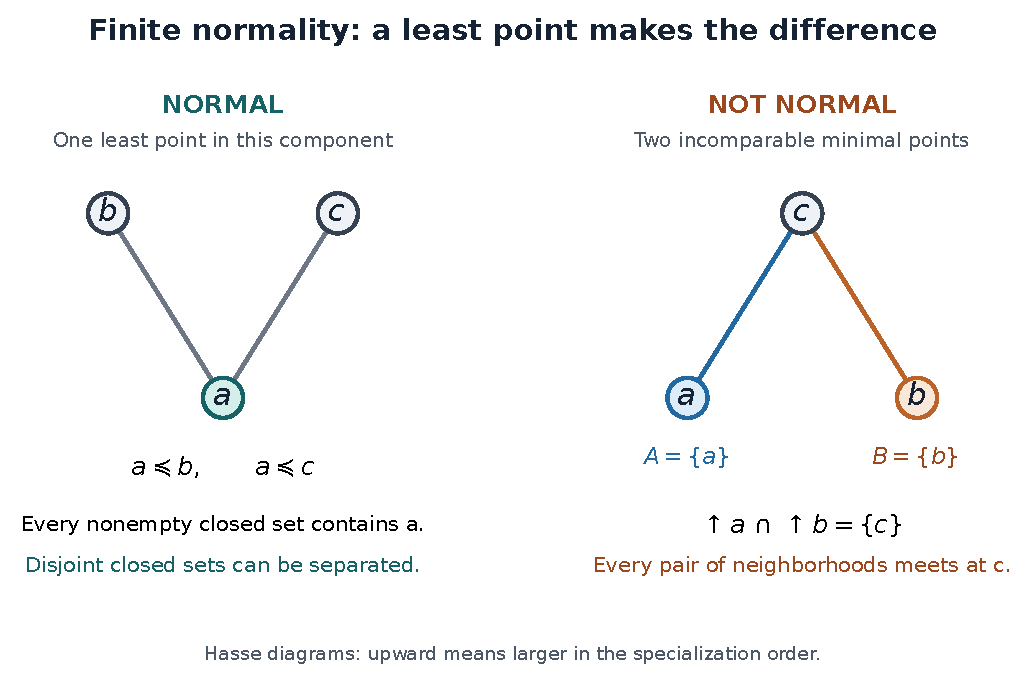
\includegraphics[width=\textwidth]{figures/finite_normality.pdf}
\caption{Open sets are upward closed. On the left, the least point $a$ lies in every nonempty closed set, so the space is normal. On the right, the disjoint closed sets $\{a\}$ and $\{b\}$ have least neighborhoods meeting at $c$; disjoint open neighborhoods and Urysohn separators do not exist.}
\label{fig:finite-normality}
\end{figure}

\subsection{Function spaces and discrete families}

\begin{theorem}[F23: finite compact-open topology and the exponential law]\label{thm:finite-exponential}
Let $C(X,Y)$ be the finite set of monotone tables between finite
spaces.  Its compact-open topology is the upward topology for
the pointwise preorder
\[
 f\preceq g\quad\Longleftrightarrow\quad
 (\forall x\in X)\ f(x)\preceq_Y g(x).
\]
Evaluation $C(X,Y)\times X\to Y$ is continuous.  For every
finite $Z$, a map $H:Z\times X\to Y$ is continuous exactly when
its curried map $z\mapsto(x\mapsto H(z,x))$ is continuous into
$C(X,Y)$.
\end{theorem}
\begin{proof}
All coded subsets $K\subseteq X$ have finite cover extraction by
F16.  The compact-open subbasic set
\[
 [K,U]=\{f:(\forall x\in K)\ f(x)\in U\}
       =\bigcap_{x\in K}[\{x\},U]
\]
is a finite intersection of point-evaluation conditions.  Each
condition is upward for pointwise order.  Conversely, the least
pointwise neighborhood of $f$ is
\[
 \mathord\uparrow f
   =\bigcap_{x\in X}[\{x\},\mathord\uparrow f(x)],
\]
which is compact-open.  Since all upward sets are unions of these
least neighborhoods, the two topologies agree.  This argument
also handles $X=\varnothing$: there is one empty map and the
empty intersection is the whole function space.

If $f\preceq g$ and $x\preceq y$, then
$f(x)\preceq g(x)\preceq g(y)$, proving evaluation monotone.
If $H$ is monotone on the product, fixing $z$ makes its section
monotone in $x$, while fixing $x$ shows pointwise monotonicity
of the curried table in $z$.  Conversely, these two monotonicity
facts give
$H(z,x)\preceq H(z',x)\preceq H(z',x')$ whenever
$(z,x)\preceq(z',x')$.  F06 translates both directions into
continuity.  Currying and uncurrying are inverse by evaluation
of their tables.  Enumerating at most $|Y|^{|X|}$ candidate
tables and testing monotonicity constructs the function-space
carrier and its pointwise relation.  Thus the proof supplies
the full finite exponential law, not only a formal analogy.
\end{proof}

\begin{theorem}[F24: finite discrete-family certificates]\label{thm:finite-discrete-family}
Given a coded indexed family $(A_i)_{i<r}$ of subsets of a finite
space, form a graph on its indices by joining distinct $i,j$
when some $x$ satisfies
\[
 \mathord\uparrow x\cap A_i\ne\varnothing,
 \qquad
 \mathord\uparrow x\cap A_j\ne\varnothing.
\]
A color class is a discrete family exactly when it contains no
graph edge.  Consequently any proper coloring supplies an
explicit decomposition into discrete families, and the greedy
algorithm always supplies at most $r$ classes.  The whole finite
family is locally finite with the uniform bound $r$.
\end{theorem}
\begin{proof}
A family is discrete when each point has an open neighborhood
meeting at most one indexed member.  Because
$\mathord\uparrow x$ is the least neighborhood of $x$, such a
neighborhood exists exactly when this least neighborhood already
meets at most one member.  Failure for a color class is exactly
an edge between two of its indices, proving the characterization.
For greedy coloring, process indices in order and choose the
least of $r$ colors absent from already colored neighbors.
At stage $i<r$ at most $i$ colors are forbidden, so a color
exists; every edge is checked when its later endpoint is colored.
Every neighborhood meets at most the $r$ indexed sets, proving
local finiteness.  Padding a finite color list by empty families
gives a certified finite instance of sigma-discreteness and
sigma-local finiteness.  No assertion about decomposing an
arbitrary infinite family follows from this finite construction.
\end{proof}

\subsection{Arithmetic proof discipline and Lean completion plan}

The algorithms above use only bounded masks, table lookup, bounded
minimum search, finite sums/products, and bounded iteration.
Their correctness proofs can be expressed with quantifier-free
Boolean invariants in \ipra.  For example, a union fold carries
the invariant that a bit is set exactly when one of the processed
sets has that bit; reachability expansion carries the invariant
that the current mask consists of vertices reachable by paths of
at most the current length.  A path code has a primitive recursive
size bound $n^{n+1}$, and removing a repeated vertex shortens its
length while preserving its endpoints.  The no-repetition
argument is finite counting on a list and is proved by bounded
induction.  A descending chain in F18 uses the same distinct-list
bound.  The elementary pigeonhole step can be verified by counting
bits, so it imports no unbounded well-foundedness principle.

For F19, use the primitive recursive predicates
$\mathrm{Preord}(n,r)$, $\mathrm{Normal}(n,r)$,
$\mathrm{Closed}(n,r,a)$, and a primitive recursive separator
constructor $s(n,r,a,b)$.  Its arithmetical assertion is
\[
\begin{split}
 &\mathrm{Preord}(n,r)\land\mathrm{Normal}(n,r)\\
 &\quad\land\mathrm{Closed}(n,r,a)\land\mathrm{Closed}(n,r,b)
 \land(a\cap b=0)\\
 &\hspace{12mm}\Longrightarrow
 \mathrm{Sep}_{01}(n,r,a,b,s(n,r,a,b)).
\end{split}
\]
Here set intersection is the bitwise primitive recursive function,
and $\mathrm{Sep}_{01}$ is the bounded test for constancy along
order pairs and for the endpoint values on the two masks.  Each
other theorem has the same shape: validity of finite input codes
implies validity of explicitly constructed output codes.  This
explains the intended first-order interpretation without claiming
that a Lean theorem about arbitrary predicates has itself already
been compiled into a checked first-order derivation.

The supplied \texttt{lean/FiniteTopology.lean} imports only
\texttt{Init}.  It defines \texttt{CPreorder}, upward and downward
predicates, interior, closure, exterior, monotone and continuous
maps, product preorders, map-space preorders, evaluation, currying,
uncurrying, and finite Boolean-table adapters.  Its checked lemmas
prove the central constructive implications in F01, F03--F04,
F06--F07, F10, and F23.  They include
\texttt{continuous\_iff\_monotone},
\texttt{closure\_idempotent},
\texttt{exterior\_iff\_not\_closure}, and the two pointwise
curry--uncurry identities.  The logged axiom audits for these
five statements report no axioms.  The file contains no admitted
proofs.  It deliberately proves the first complement identity
constructively for arbitrary predicates and leaves the converse
De Morgan identity to the decidable finite layer.

A complete formalization of this chapter has the following
concrete remaining stages.
\begin{enumerate}
\item Implement natural-number bitmask and mixed-radix encodings,
      their Boolean bounded quantifiers, and the proof that table
      decoding agrees with \texttt{Fin n} membership.  Prove the
      primitive recursive defining equations in the chosen
      ProveIt arithmetic syntax.
\item Formalize binary-fold topology tables, prove F02 by the
      explicit minimal-neighborhood construction, and specialize
      the checked order-theoretic kernel to these tables.
\item Implement Warshall closure and component expansion with the
      bounded path invariants stated above.  Use these to prove
      F11--F14 and the canonical $T_0$ quotient.
\item Prove the finite distinct-list bound and the normality
      characterization F18.  The Boolean separator in F19 and
      rational table extension in F20 then follow by component
      constancy.  These are genuine remaining proof obligations,
      not axioms supplied to make an endpoint type-check.
\item Check the rational metric tables and function-space
      enumerator, and transport the already checked evaluation
      and currying lemmas to the encoded carrier.  Finish the
      discrete-family graph criterion and bounded coloring proof.
\item Compile the resulting finite invariant proofs into explicit
      \ipra\ derivations, and run the object-theory proof checker.
      Until this final step is implemented, the artifact is a
      checked Lean kernel plus a detailed \ipra\ proof plan, not
      a completed kernel-checked formalization in the object theory.
\end{enumerate}

The independent standard-library Python checker exhaustively
examines all preorders on carriers of size $0$ through $4$;
their counts are $1,1,4,29,355$.  It independently enumerates
topology tables through size $3$, checks $92\,805$
closure/interior pairs, $24\,907$ map tables, $391$ quotient
instances, and $36$ compact-open exponentials.  It also checks
$4\,133$ two-valued separators and $7\,688$ rational-valued
extension instances (using the value alphabet $\{0,1,2\}$).
The exact results are in \texttt{data/finite\_coverage.json}.
These finite checks catch orientation, coding, and statement errors;
the uniform mathematical justification is the proofs above.
